\chapter{Material Constitutive Model}

%%%%%%%%%%%%%%%%%%%%  SECTION 1 %%%%%%%%%%%%%%%%%%%%%%%%%%%%%%%%
\section{Introduction}\label{section:CH3-S1}
%%%%%%%%%%%%%%%%%%%%%%%%%%%%%%%%%%%%%%%%%%%%%%%%%%%%%%%%%%%%%%%%

In this chapter we introduce an algorithm for shear-axial-flexure interaction 
suited for fibre beam elements of any kind (displacement-based or otherwise). 
The coupling is taken into account by considering a multiaxial constitutive law 
at the level of cross-section fibers. Thus, stress resultant interaction as 
well as the consistent tangent stiffness of a cross-section are derived during 
the state determination phase. Integration of the elastoplasic rate equations 
on each fiber is carried out using the fully backward (implicit) Euler method, 
which as is known, results in the so-called closest point projection algorithm. 
In addition, the constrained stress state of a fiber is exploited in order to 
devise a return-mapping scheme that avoids incorporating stress components that 
are not energetically active. The appropriate mapping on the constrained space 
is inspirited by the work of Simo\cite{Simo1986} and appropriately adapted for 
fibre 
discretized elements. This leads to a stress update algorithm that is 
significantly faster while also requiring less memory requirements for storage 
of non-active tensor components, compared to formulations that utilize a 
general three 
dimensional 
algorithm\cite{Papachristidis2010,Saritas2009,Ceresa2009,Gregori2007,Kagermanov2017}.
 In the latter case, stress update is a nested 
procedure within an outer Newton iteration which is necessitated in order to 
enforce the constraint for the transverse stress components, $\sigma_{22}=\ 
\sigma_{33}=0$. This is because during the trial phase of a plastic step, the 
transverse components become non-zero. Furthermore, a static condensation of 
the three-dimensional consistent tangent is required to enforce both the local 
Newton scheme and to derive the consistent tangent modulus pertaining to the 
fiber stress state. The algorithm introduced in this chapter bypasses the need 
for additional outer iterations, thereby resulting in a much faster stress 
update 
procedure.

For the exposition we adopted the $J2$ consitutive model which is based on the 
von Mises yield criterion, which is suited for modelling the elastoplastic 
response of metals. Linear kinematic and general isotropic hardening are 
incorporated in the formulation. Moreover, infinitesimal strains and a 
rate-independent associative plasticity framework are the core assumptions that 
underlie the proposed algorithm. This chapter is subdivided in three main 
sections: first, we briefly outline the general (rate) form of the 
three-dimensional elastoplastic equations. In the second section we present the 
rate constitutive model as it pertains to the fiber stress state and derive 
expressions for the continuous elastoplastic moduli. Finally, in the third 
section we outline the implementation details, which are based on application 
of the fully implicit Euler scheme. In addition we derive the expression for 
the consistent tangent modulus at a fiber, which is required to ensure 
quadratic rates of convergence for the global Newton method.

\subsection{Notation}
Furthermore, boldface lowercase letters indicate second order tensor. Wherever 
the same letters appear with an overhead arrow, this indicates the vector 
notation for the tensor represented with that letter. The notation adopted 
herein is the following:
\begin{equation*}
	\boldsymbol{\sigma} = \begin{bmatrix}
		\sigma_{11} & \sigma_{12} & \sigma_{13} \\
		\sigma_{12} & \sigma_{22} & \sigma_{23} \\
		\sigma_{13} & \sigma_{23} & \sigma_{33} \\
	\end{bmatrix}\rightarrow \bvec{\sigma} = \begin{bmatrix}
	\sigma_{11} & \sigma_{22} & \sigma_{33} & \sigma_{12} & \sigma_{23} & 
	\sigma_{13}
\end{bmatrix}^T
\end{equation*}

For strain tensors, components for which $i\neq j$ are multiplied by 2.

%%%%%%%%%%%%%%%%%%%%  SECTION 2 %%%%%%%%%%%%%%%%%%%%%%%%%%%%%%%%
\section{Three-dimensional Constitutive Model}\label{section:CH3-S2}
%%%%%%%%%%%%%%%%%%%%%%%%%%%%%%%%%%%%%%%%%%%%%%%%%%%%%%%%%%%%%%%%
Below we outline the general rate form of rate-independent elastoplasticity 
with combined isotropic and linear kinematic hardening. Infinitesimal strains 
and associateive plasticity are assumed, while the yield criterion is 
purposefully unspecified at this state in order to maintain generality. 

Let $\bm{\sigma},\ \bm{\epsilon}$ be the second order symmetric stress and 
strain tensors. We introduce the internal hardening variables $\bm{\alpha}$ and 
$q$ which represent the second order back-stress tensor and the equivalent 
uniaxial yield stress respectively. The former is associated with kinematic 
hardening while the latter models isotropic hardening. Finally, consider the 
decomposition of the strain tensor into elastic and plastic parts as follows:
\begin{equation}
	\bm{\epsilon} = \bm{\epsilon}^{el} + \bm{\epsilon}^{pl}
	\label{eq:DECOMP_STRAIN}
\end{equation} 

Then the rate form of the constitutive equations for the assumptions mentioned 
above is the following:
\begin{subequations}
	\begin{alignat}{3}
		&\dot{\bm{\epsilon}} &&= \dot{\bm{\epsilon}}^{el} +
		\dot{\bm{\epsilon}}^{pl}\quad& \text{(Strain 
		decomposition)}\label{eq:RATE_DECOMP}\\
		&\dot{\bm{\sigma}} &&= \mathbb{C}^{el}\left[\dot{\bm{\epsilon}} -
		\dot{\bm{\epsilon}}^{pl} \right]\quad& \text{(Elastic constitutive 
		law)}\label{eq:CONSTITUTIVE_LAW}\\
		&\dot{\bm{\epsilon}}^{pl} &&= \dot{\lambda}\frac{\partial \Phi}{\partial
			\bm{\sigma}}\quad& \text{(Flow rule)}\label{eq:FLOW_RULE}\\
		&\dot{\bm{\alpha}} &&= -\dot{\lambda}H_{kin}\frac{\partial 
		\Phi}{\partial
			\bm{\alpha}}\quad& \text{(Kinematic
			hardening law)}\label{eq:BACK_STRESS}\\
		&\dot{q} &&= \frac{\partial q}{\partial
			e^{pl}}\dot{e}^{pl}\quad& \text{(Isotropic hardening law)}
		\label{eq:CURRENT_YIELD_STRESS}\\
		&\dot{e}^{pl} &&= \dot{\lambda}\quad& \text{(Equivalent plastic 
		strain)}\label{eq:EQUIV_PLASTIC_STRAIN}\\
		&\Phi(\bm{\sigma},\bm{\alpha},e^{pl}) &&= 
		\sigma_{eq}(\bm{\sigma},\bm{\alpha}) - q(e^{pl}) \leq 0\quad&
		\text{(Yield criterion)}\label{eq:YIELD_FUNC} 
	\end{alignat}
	\label{eq:THREE_D_RATE}
\end{subequations}

In the above system of differential algebraic equations, $\lambda$ is the 
plastic
parameter, $H_{kin}$ is the kinematic hardening modulus, $\mathbb{C}^{el}$ is 
the elastic moduli, a fourth order tensor, of the material and $\sigma_{eq}$ is 
the equivalent stress, which is determined by the
yield criterion used. Furthermore, in the case of linear
isotropic hardening with modulus $H_{iso}$, the corresponding harening law (Eq. 
\ref{eq:CURRENT_YIELD_STRESS}) becomes $\dot{q} =
H_{iso}\dot{e}^{pl}$, where $e^{pl}$ is the equivalent plastic strain. Finally, 
with the inequality in Eq. (\ref{eq:YIELD_FUNC})
we define a feasible stress space. Stress points stictly satisfying the
inequality, $\Phi<0$ represent an elastic state while those that cause plastic 
flow
render $\Phi$ zero.

The so-called Karush-Kuhn-Tucker loading/unloading conditions derived from the 
underlying constrained variational problem\cite{Simo2006} can be stated as
follows:
\begin{equation}
	\Phi\leq 0,\qquad \dot{\lambda} \geq 0,\qquad \dot{\lambda}\Phi=0
	\label{eq:KKT_CONDITIONS}
\end{equation}

From these conditions we can determine the current stress state:
\begin{itemize}
	\item if $\dot{\lambda}>0$, then $\dot{\lambda}\Phi=0$ implies $\Phi=0$ 
	which 
	means 
	the state is plastic
	\item if $\Phi<0$, then $\dot{\lambda}\Phi=0$ implies $\dot{\lambda}=0$ and 
	from 
	(\ref{eq:FLOW_RULE}) we get that the state is elastic.
\end{itemize}
Since $\Phi=0$, $\dot{\lambda}>0$ when plastic loading persists, the third 
equation
in (\ref{eq:KKT_CONDITIONS}) leads to the so-called plastic consistency
condition:
\begin{equation}
	\dot{\lambda}\dot{\Phi}=0
	\label{eq:PLASTIC_CONSISTENCY_CONDITION}
\end{equation}

%%%%%%%%%%%%%%%%%%%%  SECTION 3 %%%%%%%%%%%%%%%%%%%%%%%%%%%%%%%%
\section{The \texorpdfstring{$J_2$}{text} formulation for fiber stress 
state}\label{section:CH3-S3}
%%%%%%%%%%%%%%%%%%%%%%%%%%%%%%%%%%%%%%%%%%%%%%%%%%%%%%%%%%%%%%%%

%%%%%%%%%%%%%%%%%%%%  SECTION 3 - SUBSECTION 1 %%%%%%%%%%%%%%%%%%%%%%%%%%%%%%%%
\subsection{Mapping on the constrained stress space}\label{section:CH3-S3SS1}

We begin by defining the admissible stress space for a planar beam fiber, 
$\mathcal{S}$:
\begin{equation*}
	\mathcal{S} = \{\bvec{\sigma}\in\mathbb{R}^6\ |\
	\sigma_{22}=\sigma_{33}=\sigma{23}=\sigma_{13}=0\}
\end{equation*}

\noindent The von Mises yield criterion is stated as follows:
\begin{equation}
	\Phi(J_2,e^{pl}) = \sqrt{3J_2} - q(e^{pl}) \leq 0
	\label{eq:VON_MISES_FUNC}
\end{equation}
where $J_2$
is the second invariant of the deviatoric stress tensor:
\begin{equation}
	J_2 = \frac{1}{2}\bm{\sigma}^d:\bm{\sigma}^d
	\label{eq:J2}
\end{equation}
The deviatoric part of any tensor is given by $(\ )^d=(\ 
)-\frac{1}{3}\bmat{I}\cdot\text{trace}[(\ )]$, with $\bmat{I}$ being the 
identity tensor and symbol <:> designates the contraction operator: 
$\bm{\sigma}^d:\bm{\sigma}^d = \sum_{i,j}\sigma_{ij}^d\sigma_{ij}^d$.

In the von Mises $J_2$ framework, the hydrostatic pressure cannot cause plastic
flow.
In other words, plastic deformation is due to the deviatoric components of the 
stress tensor and volume changes are caused only by elastic deformations. This
implies that trace[$\bm{\epsilon}^{pl}$]$=0$ which, coupled with Eq.
(\ref{eq:BACK_STRESS}), also leads to trace[$\bm{\alpha}^{pl}$]$=0$. This means 
that
the back stress tensor in Eq. (\ref{eq:BACK_STRESS}) deviatoric.

In active stress space $\mathcal{S}$ the yield function is 
$\Phi = \sqrt{\sigma_{11}^2 + 3\sigma_{12}^2}-q$ describes an ellipse, shown
in \ref{fig:FIG5_YIELDLOCUS}, with
semi-major and semi-minor axes $\sigma_y$, $\sqrt{3}^{}/3\sigma_y$, 
respectively.

\begin{figure}[t]
	\centering
	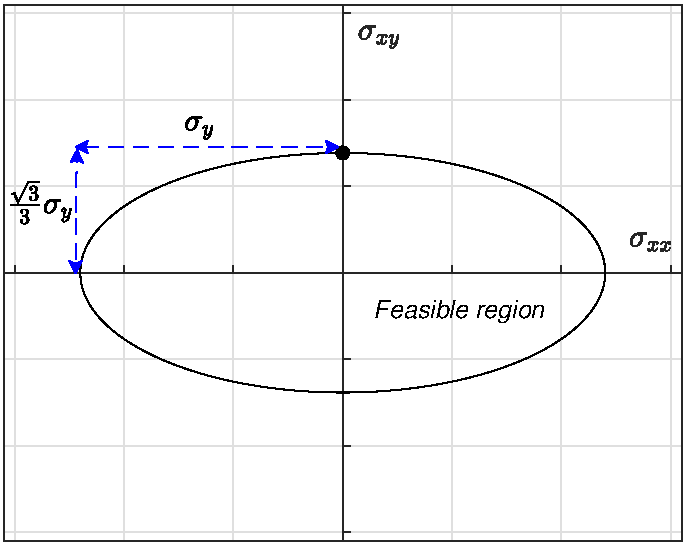
\includegraphics[scale=0.8]{FIG5_YIELDLOCUS}
	\caption{Feasible space and yield locus for the $J_2$ model. At the 
	boundary of the ellipse,
		$\sqrt{3J_2}=q$.}
	\label{fig:FIG5_YIELDLOCUS}
\end{figure}

When kinematic
hardening is included, we introduce the effective stress tensor and its
deviatoric part in order to facilitate notational simplicity:
\begin{equation}
	\bm{\zeta} = \bm{\sigma}-\bm{\alpha},\qquad \bm{\zeta}^d =
	\bm{\sigma}^d-\bm{\alpha}^d
	\label{eq:EFFECTIVE_STRESS}
\end{equation}

We now define the following vectors associated with the active tensor
components that explicitly enter subsequent derivations:
\begin{gather}
	\bvec{\alpha}_f = \begin{bmatrix} \alpha_{11} \\ \alpha_{12} 
	\end{bmatrix},\quad
	\bvec{\alpha}^d_f = \begin{bmatrix} \alpha_{11}^d \\ \alpha_{12}^d 
	\end{bmatrix},\quad
	\bvec{\epsilon}^{pl}_f = \begin{bmatrix} \epsilon^{pl}_{11} \\ 
		\gamma^{pl}_{12} \end{bmatrix},\nonumber\\
	\hspace{-0.4cm}\bvec{\sigma}^d_f = \begin{bmatrix} \sigma^d_{11} \\ 
	\sigma^d_{12}
	\end{bmatrix},\quad\hspace{0.15cm}
	\bvec{\zeta}_f = \begin{bmatrix}
		\zeta_{11} \\ \zeta_{12}
	\end{bmatrix},\quad\hspace{0.15cm}
	\bvec{\zeta}_f^d = \begin{bmatrix}
		\zeta_{11}^d \\ \zeta_{12}^d
	\end{bmatrix}\nonumber
%	\label{eq:FIBER_J2_VECTORS}
\end{gather}
The vector representation of (\ref{eq:J2}) in terms of the effective stress is:
\begin{equation}
	J_2 = \frac{1}{2}(\bvec{\zeta}^d)^T\bmat{J}\bvec{\zeta}^d 
	\label{eq:VECTOR_J2_3D}
\end{equation}
\noindent where matrix $\bmat{J} = \text{diag}[1, 1, 1, 2,2,2]$ is introduced to
account for the symmetry of $\bm{\zeta}^d$.

We now seek a mapping from the deviatoric stress space onto the fiber stress 
space $S$ of the deviatoric
effective stress vector $\bvec{\zeta}^d$ that preserves the inner product and, 
thus, the second deviatoric invariant $J_2$. The non-zero components of 
$\bvec{\zeta}^d$ are $\zeta_{11}^d,\ \zeta_{22}^d,\ \zeta_{33}^d,\
\zeta_{12}^d,\ \zeta_{21}^d$ and thus we can establish the following mappings
between the active components of $\bvec{\zeta}^d$ and $\bvec{\zeta}_f$:
\begin{equation}
	\bvec{\zeta}^d = \bmat{Q}\bvec{\zeta}_f,\qquad \bvec{\zeta}^d_f =
	\bmat{S}\bvec{\zeta}_f
	\label{eq:MAPPING}
\end{equation}
where the mapping matrices above are given by:
\begin{equation}
	\bmat{Q} = \begin{bmatrix}
		\frac{2}{3} & -\frac{1}{3} & -\frac{1}{3} & 0 & 0 & 0 \\
		0 & 0 & 0 & 1 & 0 & 0
	\end{bmatrix}^T,\qquad \bmat{S} = \begin{bmatrix}
		\frac{2}{3} & 0\\
		0 & 1
	\end{bmatrix}
	\label{eq:MAPPING_MATRIX}
\end{equation}
We can now express $J_2$ purely in terms of $\bvec{\zeta}_f$:
\begin{equation}
	J_2 = \frac{1}{2}(\bvec{\zeta}^d)^T\bmat{J}\bvec{\zeta}^d = 
	\frac{1}{2}\bvec{\zeta}_f^T\bmat{Q}^T\bmat{J}\bmat{Q}\bvec{\zeta}_f =
	\frac{1}{2}\bvec{\zeta}_f^T\bmat{V}\bvec{\zeta}_f = \frac{1}{2}\Vert
	\bvec{\zeta}_f\Vert^2_{\bm{V}}
	\label{eq:J2_EQUIV}
\end{equation}
where $\bmat{V} =\text{diag}[\frac{2}{3}, 2]$ and the notation used for the 
inner product induced by matrix $\bmat{A}$ between vectors 
$\bvec{w},\ \bvec{v}$ is $(\bvec{w},\bvec{v})_{\bm{A}} =
\bvec{w}^T\bmat{A}\bvec{v}$, which leads to the notation adopted in Eq. 
(\ref{eq:J2_EQUIV}).

With these derivations at hand, system (\ref{eq:THREE_D_RATE}) can be recast in
the constrained fiber stress state as follows:
\begin{subequations}
	\begin{alignat}{3}
		&\dot{\bvec{\epsilon}}_f &&= \dot{\bvec{\epsilon}}_f^{el} +
		\dot{\bvec{\epsilon}}_f^{pl}\quad& \text{(Strain
			decomposition)}\label{eq:FIBER_RATE_DECOMP}\\
		&\dot{\bvec{\sigma}}_f &&= \bmat{C}^{el}\left[\dot{\bvec{\epsilon}}_f -
		\dot{\bvec{\epsilon}}_f^{pl} \right]\quad& \text{(Elastic constitutive
			law)}\label{eq:FIBER_CONSTITUTIVE_LAW}\\
		&\dot{\bvec{\epsilon}}_f^{pl} &&= \dot{\lambda}\bvec{n}\quad& 
		\text{(Flow
			rule)}\label{eq:FIBER_FLOW_RULE}\\
		&\dot{\bvec{\alpha}}_f &&= 
		\dot{\lambda}H_{kin}\bmat{V}^{-1}\bvec{n}\quad& \text{(Kinematic
			hardening law)}\label{eq:FIBER_BACK_STRESS}\\
		&\dot{q}_f &&= \dot{\lambda}\frac{\partial q_f}{\partial
			e_f^{pl}}\quad& \text{(Isotropic hardening law)}
		\label{eq:FIBER_CURRENT_YIELD_STRESS}\\
		&\Phi(\bvec{\zeta}_f,e^{pl}) &&=
		\sqrt{\frac{3}{2}}\Vert\bvec{\zeta}_f\Vert_{\bm{V}} - q_f(e_f^{pl}) 
		\leq 0\quad&
		\text{(Yield criterion)}\label{eq:FIBER_J2_YIELD_FUNC} 
	\end{alignat}
	\label{eq:FIBER_RATE_SYSTEM}
\end{subequations}

\noindent Vector $\bvec{n}$ is expressed as follows:
\begin{equation}
	\bvec{n} =  \frac{\partial \Phi}{\partial \bm{\sigma}_f} = 
	- \frac{\partial \Phi}{\partial \bm{\alpha}_f} =
	\sqrt{\frac{3}{2}}\frac{\bmat{V}\bvec{\zeta}_f}{\Vert\bvec{\zeta}_f\Vert_{\bm{V}}}
	\label{eq:VECTOR_n}
\end{equation}
Equations (\ref{eq:CURRENT_YIELD_STRESS}), (\ref{eq:EQUIV_PLASTIC_STRAIN})
remain the same in the current system. In addition, note that for the 
$J_2$ model, the left-hand side of eq. (\ref{eq:BACK_STRESS}) is a deviatoric 
tensor whereas in (\ref{eq:FIBER_BACK_STRESS}) it has been mapped to fiber 
stress space $\mathcal{S}$.


%%%%%%%%%%%%%%%%%%%%  SECTION 3 - SUBSECTION 2 %%%%%%%%%%%%%%%%%%%%%%%%%%%%%%%%
\subsection{Continuous tangent modulus}\label{section:CH3-S3SS2}

The continuous elastoplastic modulus $\bmat{C}^{ep}$ is found by enforcing the
plastic consistency condition (\ref{eq:PLASTIC_CONSISTENCY_CONDITION}) during a 
plastic step:
\begin{equation}
	\bvec{n}^T\dot{\bvec{\zeta}}_f-\dot{\lambda}\frac{\partial q_f}{\partial
		e_f^{pl}} = 0
	\label{eq:FIBER_PLASTIC_CONSISTENCY_ENF}
\end{equation}
The rate form for the effective stress is given by combining Eqs.
(\ref{eq:FIBER_CONSTITUTIVE_LAW}), (\ref{eq:FIBER_BACK_STRESS}) with
$\dot{\bvec{\zeta}}_f = \dot{\bvec{\sigma}}_f - \dot{\bvec{\alpha}}_f$:
\begin{equation}
	\dot{\bvec{\zeta}}_f = \bmat{C}^{el}\dot{\epsilon}_f -
	\dot{\lambda}\bmat{Z}\bvec{n}
	\label{eq:RATE_FORM_EFFECTIVE}
\end{equation}
\noindent where $\bmat{Z} = \bmat{C}^{el}+H_{kin}\bmat{V}^{-1}$.
Substituting (\ref{eq:RATE_FORM_EFFECTIVE}) into
(\ref{eq:FIBER_PLASTIC_CONSISTENCY_ENF}) and solving for $\dot{\lambda}$ we get:
\begin{equation}
	\dot{\lambda} =
	\frac{\bvec{n}^T\bmat{C}^{el}\dot{\bvec{\epsilon}}_f}{\bvec{n}^T\bmat{Z}\bvec{n}+
		\frac{\partial q_f}{\partial e_f^{pl}}}
	\label{eq:PLASTIC_PARAM_RATE}
\end{equation}
Finally, by making use of (\ref{eq:PLASTIC_PARAM_RATE}),
(\ref{eq:FIBER_FLOW_RULE}) and (\ref{eq:FIBER_CONSTITUTIVE_LAW}), we arrive at
the expression for the continuous elastoplastic modulus:
\begin{equation}
	\bmat{C}^{pl} =
	\bmat{C}^{el}-\frac{\bvec{m}\bvec{m}^T}{\bvec{n}^T\bmat{Z}\bvec{n}+
		\frac{\partial q_f}{\partial e_f^{pl}}}
	\label{eq:CONT_ELASTOPLASTIC_MODULUS}
\end{equation}
\noindent where $\bvec{m} = \bmat{C}^{el}\bvec{n}$.

%%%%%%%%%%%%%%%%%%%%  SECTION 4 %%%%%%%%%%%%%%%%%%%%%%%%%%%%%%%%
\section{Implicit integration of rate equations}\label{section:CH3-S4}
%%%%%%%%%%%%%%%%%%%%%%%%%%%%%%%%%%%%%%%%%%%%%%%%%%%%%%%%%%%%%%%%

We employ the fully implicit backward Euler method to discretize the rate
constitutive equations in system (\ref{eq:FIBER_RATE_SYSTEM}) in the pseudotime
interval $[t_n,t_{n+1}]$. We regard the incremental/iterative process as strain
driven, in that at the start of increment $n$, the dependent state variables 
for each fiber,
$S_n=\{\bvec{\epsilon}_f,\bvec{\epsilon}_f^{pl},\bvec{\alpha}_f,e_f^{pl}\}_n$, 
are
known and stored. We also know the increment in the centerline strain vector
$\bvec{d}$, $\Delta\bvec{d}$. The incremental strain vector for the current
fiber is then determined using eq. (\ref{eq:f2}):
\begin{equation*}
	\Delta\bvec{\epsilon}_f = \bmat{N}_s\Delta\bvec{q}
	\label{eq:INCREMENTAL_STRAINS}
\end{equation*}
Given the incremental strain vector $\Delta\bvec{\epsilon}_f$, 
we need to update the state variables for $t_{n+1}$:  $S_n\rightarrow S_{n+1}$.
In what follows we ommit the subscript denoting the vector pertains to the fiber
state: 
\begin{equation*}
	S_n \equiv
	\{\bvec{\epsilon}_n,\bvec{\epsilon}_n^{pl},\bvec{\alpha}_n,e_n^{pl}\},\qquad
	S_{n+1} \equiv
	\{\bvec{\epsilon}_{n+1},\bvec{\epsilon}_{n+1}^{pl},\bvec{\alpha}_{n+1},e_{n+1}^{pl}\},
\end{equation*}

The update of the fiber total strain vector $\bvec{\epsilon}$ is trivial:
$\bvec{\epsilon}_{n+1} = \bvec{\epsilon}_n + \Delta\bvec{\epsilon}$. For the
remaining state variables the rate system (\ref{eq:FIBER_RATE_SYSTEM}) is 
discretized as follows:
\begin{subequations}
	\begin{alignat}{2}
		&\bvec{\sigma}_{n+1} &&=  
		\bmat{C}^{el}\left[\bvec{\epsilon}_{n+1} -
		\bvec{\epsilon}_{n+1}^{pl} 
		\right]\label{eq:FIBER_CONSTITUTIVE_LAW_DISCR}\\
		&\bvec{\epsilon}_{n+1}^{pl} &&= \bvec{\epsilon}_{n}^{pl} +
		\dot{\lambda}\bvec{n}_{n+1}
		\label{eq:FIBER_FLOW_RULE_DISCR}\\
		&\bvec{\alpha}_{n+1} &&=\bvec{\alpha}_{n} + 
		\lambda H_{kin}\bmat{V}^{-1}\bvec{n}_{n+1}
		\label{eq:FIBER_BACK_STRESS_DISCR}\\
		&q_{n+1} &&= q_{n} + \lambda\frac{\partial q_{n+1}}{\partial
			e_{n+1}^{pl}}\label{eq:FIBER_CURRENT_YIELD_STRESS_DISCR}\\
		&\Phi(\bvec{\zeta}_{n+1},e_{n+1}^{pl}) &&=
		\sqrt{\frac{3}{2}}\Vert\bvec{\zeta}_{n+1}\Vert_{\bm{V}} -
		q_{n+1}(e_{n+1}^{pl}) \leq 0
		\label{eq:FIBER_J2_YIELD_FUNC_DISCR}
	\end{alignat}
	\label{eq:FIBER_DISCR_SYSTEM}
\end{subequations}
\noindent and
\begin{equation}
	\bvec{\zeta}_{n+1} = \bvec{\sigma}_{n+1} - \bvec{\alpha}_{n+1}
	\label{eq:DISCR_EFFECTIVE}
\end{equation}


%%%%%%%%%%%%%%%%%%%%  SECTION 4 - SUBSECTION 1 %%%%%%%%%%%%%%%%%%%%%%%%%%%%%%%%
\subsection{Elastic predictor - Plastic Corrector 
algorithm}\label{section:CH3-S4SS1}

It is convenient to recast system (\ref{eq:FIBER_DISCR_SYSTEM})
purely in terms of stress by utilizing
(\ref{eq:DISCR_EFFECTIVE}),(\ref{eq:FIBER_CONSTITUTIVE_LAW_DISCR}),(\ref{eq:FIBER_BACK_STRESS_DISCR}):

\begin{minipage}{0.35\linewidth}
	\hspace{1.7cm}\begin{tabular}[]{c}
		\textbf{Stress rate system}\\
		\specialrule{2.pt}{1pt}{-15pt}
	\end{tabular}
	\begin{subequations}
		\begin{align}
			\dot{\bvec{\zeta}} &=
			\bmat{C}^{el}\dot{\bvec{\epsilon}}-\dot{\lambda}\bmat{Z}\bvec{n}\label{eq:EFF_RATE1}\\
			\dot{q} &= \dot{\lambda}\frac{\partial q}{\partial
				e^{pl}}\label{YIELD_RATE2}
		\end{align}
		\label{eq:REDUCED_RATE_SYS}
	\end{subequations}
\end{minipage}
\begin{minipage}{0.6\linewidth}
	\hspace{1.7cm}\begin{tabular}[]{c}
		\textbf{Discretized system}\\
		\specialrule{2.pt}{1pt}{-15pt}
	\end{tabular}
	\begin{subequations}
		\begin{align}
			\bvec{\zeta}_{n+1} &= \bvec{\zeta}_n +
			\bmat{C}^{el}\Delta\bvec{\epsilon}_{n+1}-\lambda\bmat{Z}\bvec{n}_{n+1}\label{eq:EFF_DISCR1}\\
			q_{n+1} &= q_n + \lambda\frac{\partial q_{n+1}}{\partial
				e_{n+1}^{pl}}\label{eq:YIELD_DISCR2}
		\end{align}
		\label{eq:REDUCED_DISCR_SYS}
	\end{subequations}
\end{minipage}

We need not differentiate between initial and final value for the plastic
parameter $\lambda$ since it is initialized to zero at the beginning of every
step: $\lambda_n = 0$. The solution of (\ref{eq:REDUCED_DISCR_SYS}) is based on
a two-step procedure. The first phase is called trial elastic step, where 
we assume that the increment $\Delta\bvec{\epsilon}$ is elastic and all state 
variables are updated by setting $\lambda=0$: $S_n\rightarrow S_{n+1}^{TR}$. If 
the trial stresses satisfy the yield condition $\Phi^{TR}_{n+1} < 0$, then the 
step
was indeed elastic and we can set $S^{TR}_{n+1}\rightarrow S_{n+1}$. If the 
yield 
criterion is violated, $\Phi^{TR}_{n+1}>0$, then the step is plastic and we 
need to 
apply (plastic) corrections to the state variables so that, upon convergence, 
we have achieved $\Phi_{n+1} = 0$. This procedure is referred to as
Elastic Predictor - Plastic Corrector algorithm and can be traced back to the
work of Wilkins\cite{Wilkins1963}. It has enjoyed widespread
application in solving problems in
elastoplasticity\cite{Dodds1987,DeAngelis2015,Clausen2006,Hopperstad1995,Scherzinger2017,Hartloper2021}
and the basic relations for each step are summarized below.

\hspace{-1.2cm}\begin{minipage}{0.5\linewidth}
	\hspace{1cm}\begin{tabular}[]{c}
		\textbf{Elastic Predictor}\\
		\specialrule{2.pt}{1pt}{-15pt}
	\end{tabular}
	\begin{subequations}
		\begin{align}
			\bvec{\zeta}_{n+1}^{TR} &= \bmat{C}^{el}\left[\bvec{\epsilon}_{n+1}-
			\bvec{\epsilon}_n^{pl}\right]-\bvec{\alpha}_n\label{eq:TRIAL_EFFECTIVE}\\
			q_{n+1}^{TR} &= q_n \label{eq:TRIAL_YIELD}\\
			\Phi_{n+1}^{TR} &=
			f_(\bvec{\zeta}_{n+1}^{TR},q_{n+1}^{TR})\label{eq:TRIAL_YIELDFUN}
		\end{align}
		\label{eq:ELASTIC PREDICTOR}
	\end{subequations}
\end{minipage}
\hspace{0.3cm}\begin{minipage}{0.05\linewidth}
	$\xrightarrow{\Phi_{n+1}^{TR}>0}$
\end{minipage}
\hspace{0.70cm}\begin{minipage}{0.4\linewidth}
	\hspace{1.7cm}\begin{tabular}[]{c}
		\textbf{Plastic Corrector}\\
		\specialrule{2.pt}{1pt}{-15pt}
	\end{tabular}
	\begin{subequations}
		\begin{align}
			\bvec{\zeta}_{n+1} &= \bvec{\zeta}_{n+1}^{TR} - 
			\lambda\bmat{Z}\bvec{n}_{n+1}\label{eq:CORRECTOR_EFFECTIVE}\\
			q_{n+1} &= q_{n+1}^{TR} + \lambda\frac{\partial q_{n+1}}{\partial
				e_{n+1}^{pl}}\label{eq:CORRECTOR_YIELD}\\
			\Phi_{n+1} &= 0\label{eq:CORRECTOR_YIELDFUN}
		\end{align}
		\label{eq:PLASTIC CORRECTOR}
	\end{subequations}
	\label{eq:PLASTIC_CORRECTOR_SYS}
\end{minipage}

The Plastic Corrector step is a system of 4 nonlinear algebraic equations with 
4 unknowns, $\{\zeta_{11,n+1}, \zeta_{12,n+1}, q_{n+1}, \lambda\}$, and
generally a local Newton method is required to determined the unknowns. It
should be stressed here that, in multiaxial constitutive algorithms that do not
make use of the mapping as developed here, this local process is nested within 
an upper level Newton procedure that enforces the zero transverse
stress condition.

Substituting Eqs. (\ref{eq:CORRECTOR_EFFECTIVE}),(\ref{eq:CORRECTOR_YIELD})
into (\ref{eq:CORRECTOR_YIELDFUN}) furnishes a nonlinear scalar equation that
needs to be solved for $\lambda$. Once $\lambda$ is computed, then the fiber
state can be updated $S_{n+1}^{TR}\rightarrow S_{n+1}$. Refer also to
Box ~\ref{Box:BOX1} for a detailed summary of the plastic updates. Detailed
expressions for the local Newton method on $\Phi_{n+1}(\lambda)=0$ are provided 
in Appendix \ref{appendix:APPENDIX_C}.

%%%%%%%%%%%%%%%%%%%%  SECTION 4 - SUBSECTION 2 %%%%%%%%%%%%%%%%%%%%%%%%%%%%%%%%
\subsection{Consistent Tangent Modulus}\label{section:CH3-S4SS2}

The tangent modulus consistent with the numerical discretization used on system
(\ref{eq:FIBER_RATE_SYSTEM}) is necessary to restore the quadratic rates of
convergence for the global Newton method\cite{Simo1985}. That is:
\begin{equation}
	\bmat{C}_c^{pl} =
	\frac{\text{d}\bvec{\sigma}_{n+1}}{\text{d}\bvec{\epsilon}_{n+1}}
	\label{eq:CONSISTENT_TANG_FORM}
\end{equation}
We take the differentials of (\ref{eq:FIBER_CONSTITUTIVE_LAW_DISCR}),
(\ref{eq:FIBER_BACK_STRESS_DISCR}) and (\ref{eq:FIBER_J2_YIELD_FUNC_DISCR}), 
using the fact that 
$\text{d}\bvec{\zeta}_{n+1} = \text{d}\bvec{\sigma}_{n+1} -
\text{d}\bvec{\alpha}_{n+1}$ from (\ref{eq:DISCR_EFFECTIVE}) and arrive at the
following system:
\begin{subequations}
	\begin{equation}
		\begin{bmatrix}
			\bmat{C}^{el}+\lambda\bmat{B}_{n+1} & -\lambda\bmat{B}_{n+1}\\
			-\lambda\bmat{B}_{n+1} & H_{kin}^{-1}\bmat{V}+\lambda\bmat{B}_{n+1}
		\end{bmatrix}\begin{bmatrix}
			\text{d}\bvec{\sigma}_{n+1}\\
			\text{d}\bvec{\alpha}_{n+1}
		\end{bmatrix} = \begin{bmatrix}
			\text{d}\bvec{\epsilon}_{n+1}-\text{d}\lambda\bvec{n}_{n+1}\\
			\text{d}\lambda\bvec{n}_{n+1}
		\end{bmatrix}
		\label{eq:DIFF_SYSTEM}
	\end{equation}
	\begin{equation}
		\bvec{n}_{n+1}^T\left[\text{d}\bvec{\sigma}_{n+1} -
		\text{d}\bvec{\alpha}_{n+1}\right] = \text{d}\lambda
		\frac{\partial q_{n+1}}{\partial e_{n+1}^{pl}}
		\label{eq:YIELD_FUNC_DIFF}
	\end{equation}
	\label{eq:DIFF_SYS_YIELD}
\end{subequations}

\noindent where $\bmat{B}$ is given as follows:
\begin{equation}
	\bmat{B} = \frac{\partial\bvec{n}}{\partial \bvec{\zeta}}=
	\frac{\partial^2 f}{\partial \bvec{\zeta}^2} = \frac{1}{\Vert
		\bvec{\zeta}\Vert_{\bm{V}}}\left[ \bmat{V}-\bvec{n}\bvec{n}^T\right]
	\label{eq:B}
\end{equation}
Upon solving (\ref{eq:DIFF_SYSTEM}) for $\text{d}\bvec{\sigma}_{n+1}$,
$\text{d}\bvec{\alpha}_{n+1}$ we substitute them into (\ref{eq:YIELD_FUNC_DIFF})
and solve for d$\lambda$:
\begin{equation}
	\text{d}\lambda =
	\frac{\bvec{n}_{n+1}^T\left[\bmat{\Xi}_{11}+\bmat{\Xi}_{12}^T\right]\text{d}\bvec{\epsilon}_{n+1}}{\bvec{n}_{n+1}^T\bmat{T}\bvec{n}_{n+1}+
		\frac{\partial q_{n+1}}{\partial e_{n+1}^{pl}}}
	\label{eq:DE_GAMMA}
\end{equation}
Finally, substituting d$\lambda$ into (\ref{eq:FIBER_CONSTITUTIVE_LAW_DISCR}) 
furnishes the formula for the consistent tangent modulus:
\begin{equation}
	\bmat{C}_c^{pl} = 
	\bmat{\Xi}_{11}-\frac{\bvec{N}_{n+1}\bvec{N}_{n+1}^T}{1+\delta_{n+1}}
	\label{eq:CONSISTENT TANGENT MOD}
\end{equation}
Details regarding all newly defined vectors and matrices involved in the
derivation of $\bmat{C}_c^{pl}$ is given in Appendix \ref{appendix:APPENDIX_D}. 
In Box ~\ref{Box:BOX1} 
we have summarised the return mapping algorithnm for a fiber.

%%%%%%%%%%%%%%%%%%%%  SECTION 4 - SUBSECTION 3 %%%%%%%%%%%%%%%%%%%%%%%%%%%%%%%%
\subsection{Consistent Section Stiffness}\label{section:CH3-S4SS3}

Once the stress update on a particular fiber has been carried out, its
contribution to the stress resultant vector and the section stiffness are
accounted for via a midpoint integration rule along the section height (see Eqs.
(\ref{eq:STRESS_RES_CONJUGATE}), (\ref{eq:FIB_STIFF_CONTRIB}).

Notice that while in the present formulation $C_{21}=C_{12}$, this will not be
the case if a generalized integration rule is used for the rate equations. In
such a scenario, if enforcement of the plastic consistency does not correspond
to the interior time $t_a\in[t_n, t_{n+1}]$ chosen, that is $\Phi_a=0$, then 
the consistenttangent will not be symmetric. For more details on this refer to
\cite{Ortiz1985}.

% ~~~~~~~~~~~~~~~~~~~~~~ BOX 1  ~~~~~~~~~~~~~~~~~~~~~``
{
	\centering
	\begin{tcolorbox}[tikznode boxed title,enhanced,arc=0mm,interior
		style={white}, colbacktitle=white,coltitle=black,
		width=5in,top=5pt,bottom=10pt,boxrule=1pt,toprule=1pt,fonttitle=\bfseries,title={Box
		 1
			: Summary of Elastic Predictor - Plastic Corrector 
			algorithm.},sharp corners,
		boxed title style = {size=normal,colframe=white,boxrule=0pt}]
		$\bullet\hspace{0.5cm}$  \textbf{Start of step - Elastic Predictor}
		
		\vspace{-1.2cm}
		\begin{minipage}[t]{0.6\linewidth}
			\begin{alignat*}{2}
				\blacksquare\hspace{0.3cm}	&\bvec{\epsilon}^{pl,TR}_{n+1} &&= 
				\bvec{\epsilon}^{pl}_n\\
				\blacksquare\hspace{0.3cm}	&\bvec{\sigma}^{TR}_{n+1} &&=
				\bmat{C}^{el}\left[\bvec{\epsilon}_{n+1}-\bvec{\epsilon}^{pl}_n\right]\\
				\blacksquare\hspace{0.3cm}	&\bvec{\alpha}^{TR}_{n+1} &&= 
				\bvec{\alpha}_n\\
			\end{alignat*}
		\end{minipage}
		\begin{minipage}[t]{0.22\linewidth}
			\begin{alignat*}{2}
				\blacksquare\hspace{0.3cm} &e^{pl,TR}_{n+1} &&= e^{pl}_n\\
				\blacksquare\hspace{0.3cm}	&q^{TR}_{n+1} &&= q_n\\
				\blacksquare\hspace{0.3cm}	&f_{n+1}^{TR} &&=
				\Phi(\bvec{\zeta}_{n+1}^{TR},q_{n+1}^{TR})
			\end{alignat*}
		\end{minipage}
		
		\vspace{-0.3cm}
		$\bullet\hspace{0.5cm}\text{IF}\ \Phi_{n+1}^{TR}<0\rightarrow$  
		\textbf{Elastic Step}
		
		\vspace{-1.2cm}
		\hspace{-1.03cm}\begin{minipage}[t]{0.6\linewidth}
			\begin{alignat*}{2}
				\blacksquare\hspace{0.3cm}	&\bvec{\epsilon}^{pl}_{n+1} &&=
				\bvec{\epsilon}^{pl,TR}_{n+1}\\
				\blacksquare\hspace{0.3cm}	&\bvec{\sigma}_{n+1}
				&&=\bvec{\sigma}^{TR}_{n+1}\\
				\blacksquare\hspace{0.3cm}	&\bvec{\alpha}_{n+1} &&= 
				\bvec{\alpha}^{TR}_{n+1}
			\end{alignat*}
		\end{minipage}
		\begin{minipage}[t]{0.41\linewidth}
			\begin{alignat*}{2}
				\blacksquare\hspace{0.3cm} &e^{pl}_{n+1} &&= e^{pl,TR}_{n+1}\\
				\blacksquare\hspace{0.3cm}	&q_{n+1} &&= q^{TR}_{n+1}\\
				\blacksquare\hspace{0.3cm}	&\bmat{C} &&= \bmat{C}^{el}
			\end{alignat*}
		\end{minipage}
		
		\vspace{0.6cm}
		$\bullet\hspace{0.5cm}\text{ELSE}\ f_{n+1}^{TR}>0\rightarrow$  
		\textbf{Plastic Corrector}
		\begin{enumerate}
			\item Iteratively solve (\ref{eq:PLASTIC_CORRECTOR_SYS}) for 
			$\lambda$:
			$\lambda^{j+1}=\lambda^j-\frac{\Phi_{n+1}^j}{(\frac{\text{d}\Phi_{n+1}}{\text{d}\lambda})^j}$,
			with $\lambda^0 = 0$, $\Phi_{n+1}^0 = \Phi_{n+1}^{TR}$. Loop 
			termination:
			$|\Phi_{n+1}^{j+1}|\leq e_{tol}$, where $e_{tol}$ small.
			\item Update state variables:
			
			\vspace{-1.7cm}
			\hspace{-0.15cm}\begin{minipage}[t]{0.3\linewidth}
				\begin{alignat*}{2}
					\blacksquare\hspace{0.3cm}	&\bvec{\zeta}_{n+1} &&=
					[\bm{\Omega}(\lambda)]\bvec{\zeta}_{n+1}^{TR}\\
					\blacksquare\hspace{0.3cm}	&\bvec{\epsilon}^{pl}_{n+1} &&= 
					\bvec{\epsilon}^{pl}_n + \lambda\bvec{n}_{n+1}\\
					\blacksquare\hspace{0.3cm}	&\bvec{\alpha}_{n+1} &&= 
					\bvec{\alpha}_n + \lambda 
					H_{kin}\bmat{V}^{-1}\bvec{n}_{n+1}\\
				\end{alignat*}
			\end{minipage}
			\begin{minipage}[t]{0.4\linewidth}
				\begin{alignat*}{2}
					\blacksquare\hspace{0.3cm} &\bvec{\sigma}_{n+1} &&= 
					\bvec{\zeta}_{n+1} + \bvec{\alpha}_{n+1}\\
					\blacksquare\hspace{0.3cm} &e^{pl}_{n+1} &&= e^{pl}_n + 
					\lambda \\
					\blacksquare\hspace{0.3cm}	&q_{n+1} &&= q_n + 
					\lambda\frac{\partial
						q_{n+1}}{\partial e_{n+1}^{pl}}
				\end{alignat*}
			\end{minipage}
			
			\vspace{-0.5cm}
			\item Get consistent tangent modulus
			\vspace{-0.5cm}
			$$\bmat{C}=\bmat{C}_c^{pl} = 
			\bmat{\Xi}_{11}-\frac{\bvec{N}_{n+1}\bvec{N}_{n+1}^T}{1+\delta_{n+1}}$$
		\end{enumerate}
		See Appendix \ref{appendix:APPENDIX_C} for $[\bm{\Omega}(\lambda)]$.
		\step\label{Box:BOX1}
	\end{tcolorbox}
}


